%Kaptitel 1

\chapter{Aufgabe D5}
Die untenstehende \autoref{fig:Simulink5} zeigt den "Random Number Generator". \\
Die Daten werden nach der Vorschrift$$ X(i) = (a*X(i-1)+c)\mod m$$ generiert.\\
Die Parameter a, c und m sowie X(0) sind hierfür frei wählbar, um optimale Zufallsazahlen zu erhalten.\\
Dafür sind einige Vorschriften zu beachten:\\ 
$ Modul \thinspace {\displaystyle m\in \{2,3,4,\ldots \}} \\
\thinspace Faktoren\thinspace {\displaystyle a_{1},\ldots ,a_{n}\in \left\{0,\ldots ,m-1\right\}}\thinspace mit \thinspace{\displaystyle a_{n}>0}\\
Inkrement\thinspace {\displaystyle b\in \left\{0,\ldots ,m-1\right\}}\\
Startwerte \thinspace{\displaystyle y_{1},\ldots ,y_{n}\in \left\{0,\ldots ,m-1\right\}} \hspace{1cm}(nicht\thinspace alle\thinspace\thinspace 0, \thinspace wenn\thinspace {\displaystyle b=0} )
$\\

Nach diesen Vorschriften wurde a = 89 und c = 253 gewählt. Beide Zahlen sind Primzahlen und haben somit keinen gemeinsamen Teiler mit m = $2\textsuperscript{31}$.
m als Zweierpotenz zu wählen ist besonders effizient, da so die Modulooperation durch das abschneiden der Zahl in Binärdarstellung berechnet werden kann.\\
Für $c \neq 0$ muss außerdem folgendes gelten, damit m Zufallszahlen bei einem beliebigen Seed generiert werden:\\
1. m und c haben keinen gemeinsamen Teiler\\
2. a - 1 ist durch alle Primfaktoren von m teilbar\\
3. a - 1 durch 4 teilbar wenn  m durch 4 teilbar ist\\
Die zusätzlichen  Anforderungen werden von den gewählten Parametern erfüllt. Zur Generierung von 4 Datensätzen werden unterschiedliche Startwerte X(0) gewählt.
Die Rechenoperation wurde darüber hinaus noch ergänzt. Wie in \autoref{fig:Simulink5} dargestellt wird die nach der Generierung der Zufallszahl nach obengenannter Vorschrift, noch die Hälfte von m subtrahiert, um auch negative Zufallswerte zu erhalten. Des Weiteren wird danach die Zufallszahl noch mit einem Wert multipliziert, um die Amplitude, um die die Zufallszahlen um 0 oszillieren zu setzen. Abschließend wird noch ein Zielwert addiert, um die Zufallszahlen um einen Zielwert oszillieren zu lassen.

\begin{figure}[H]
	\centering
	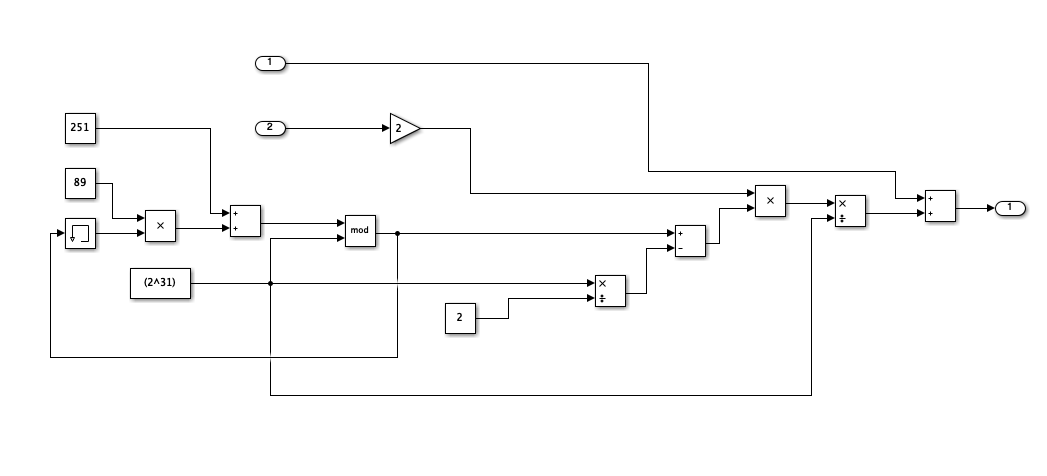
\includegraphics[width=1\linewidth]{../Graphiken/Simulink5}
	\caption{Random Number Generator}
	\label{fig:Simulink5}
\end{figure}